\chapter{ Констукторский раздел}
\label{cha:design}

\section{Требования к программе}

Программа должна предоставлять следующие возможности:
\begin{enumerate}
	\item Визуализацию сцены.
	\item Запуск системы.
	\item Останов системы.
\end{enumerate}

\section{Алгоритм обратной трассировки лучей}

Рассмотрим схему алгоритма (\ref{fig:ref3}). В данном проекте алгоритм обратной трассировки лучей будет применяться к шару, для того, чтобы воспользоваться данным алгоритмом нам нужно уметь находить пересечение луча и сферы.

\begin{figure}[ht!]
	\centering{
		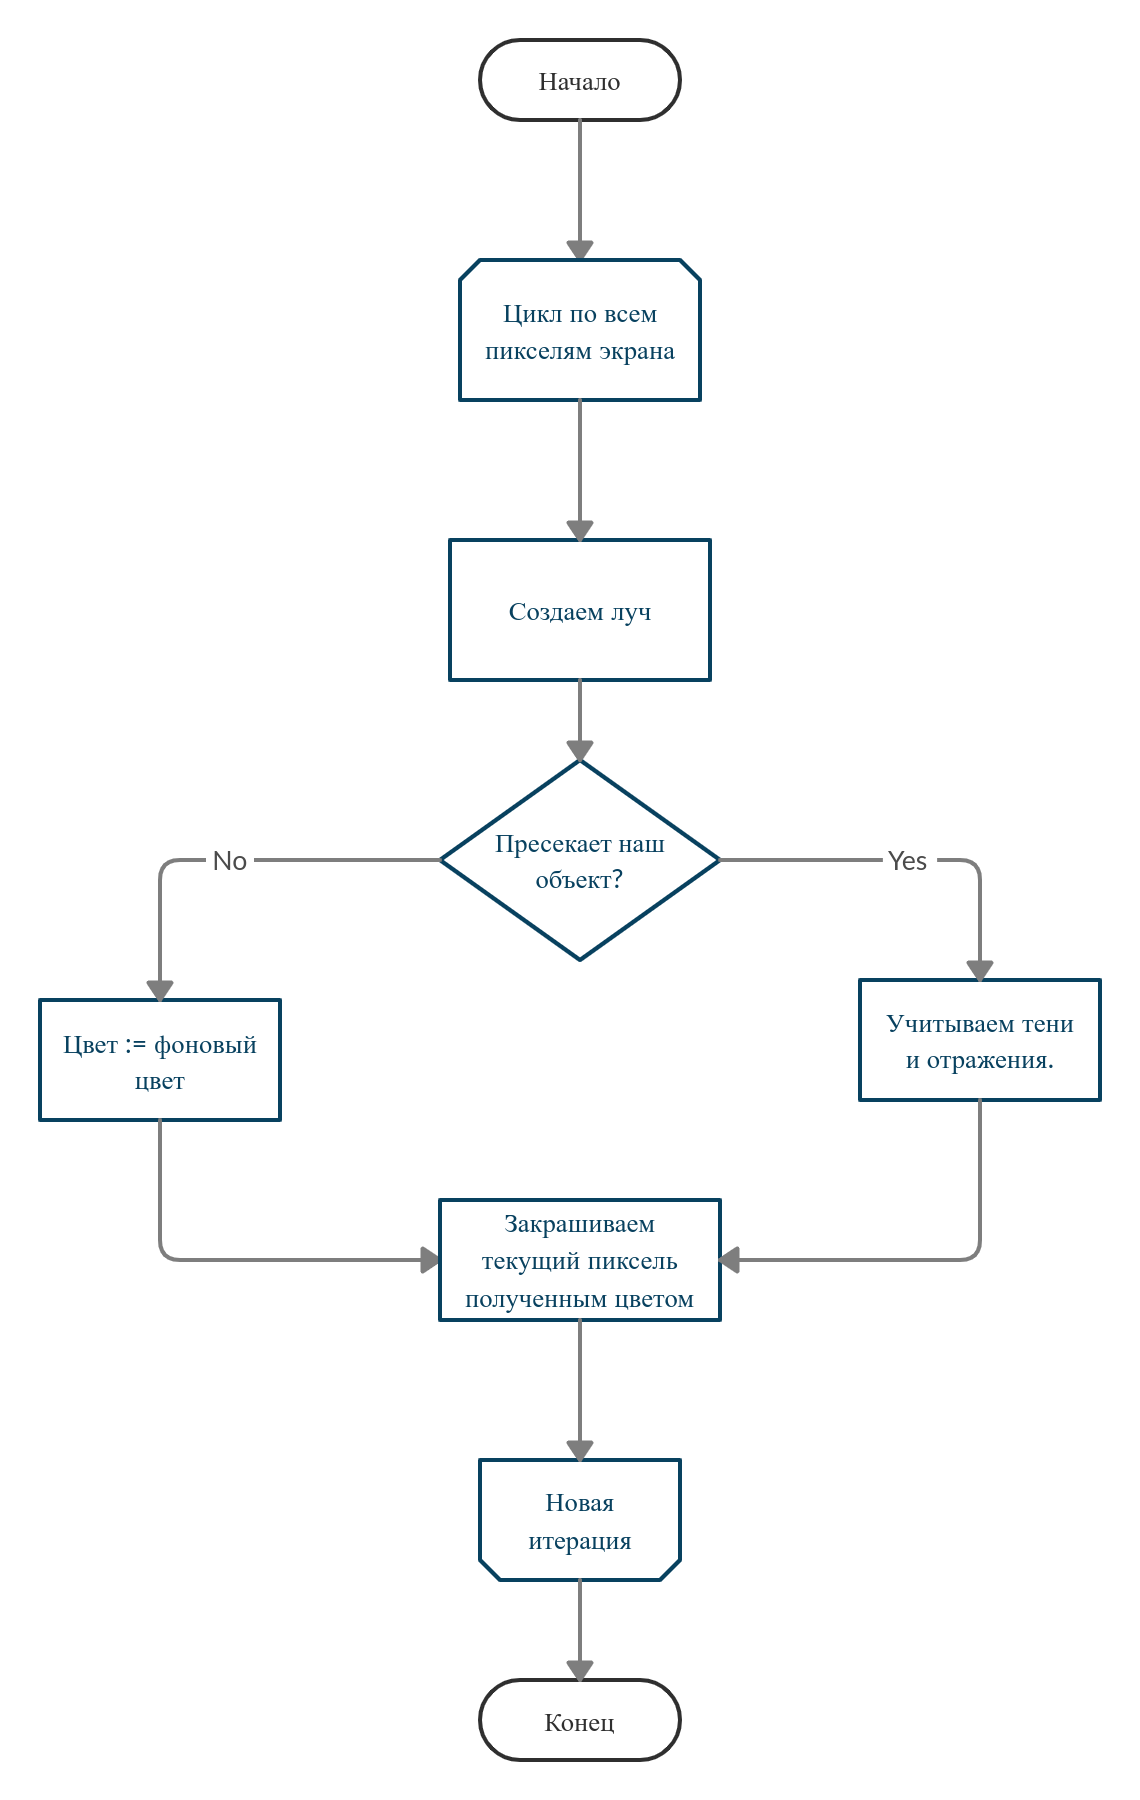
\includegraphics[width=0.6\textwidth]{img/block_diagram.png}
		\caption{Блок-схема алгоритма трассировки лучей}
		\label{fig:ref3}}
\end{figure}

Уравнение луча представлено ниже:

\begin{equation}
	P = O + t(V - O)
	\label{eq:ref5}
\end{equation}

Где О - центр камеры, а V - текущий пиксель.

Обозначим направление луча:

\begin{equation}
	\overrightarrow{D} = V - O
\end{equation}

Рассмотрим, что из себя представляет сфера.

%\begin{figure}[ht!]
%	\centering{
%		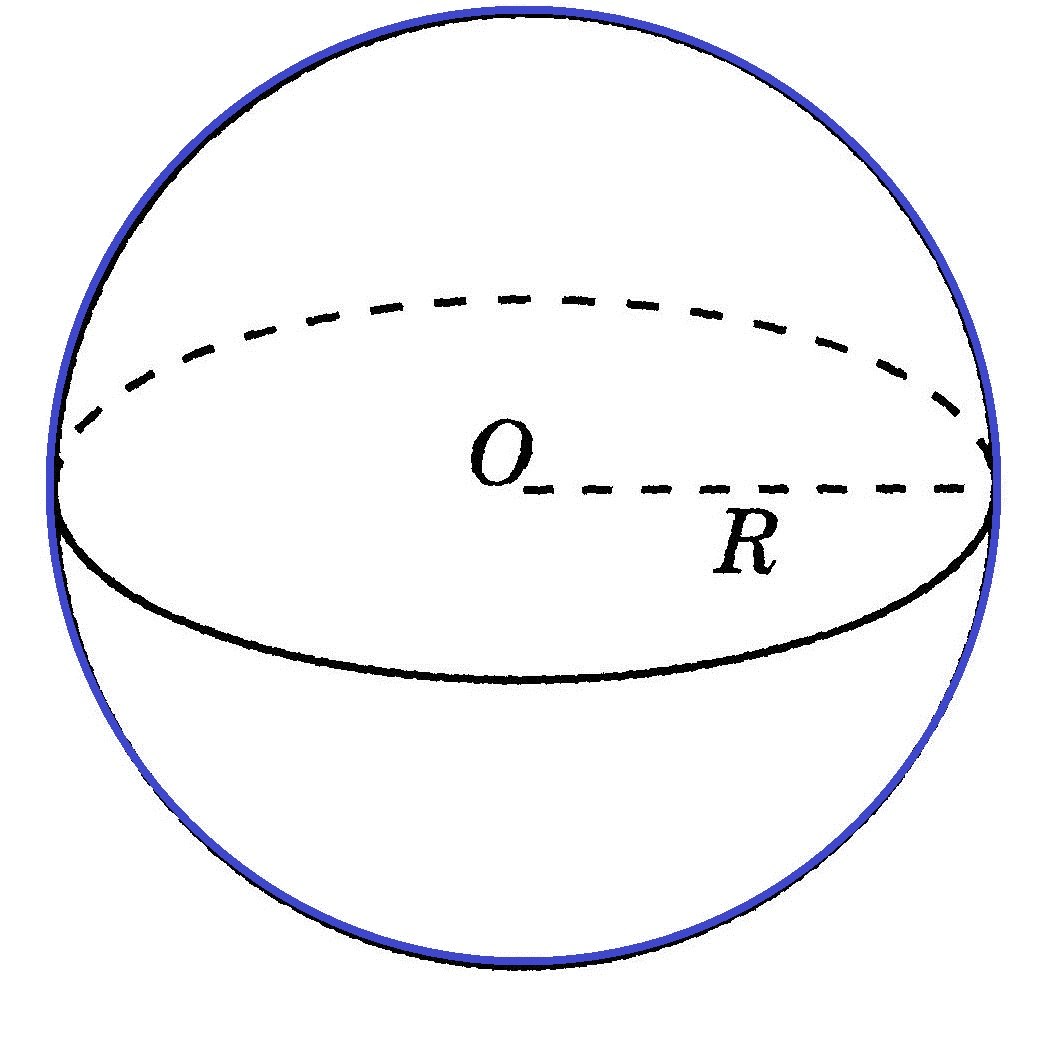
\includegraphics[width=0.5\textwidth]{img/sphere.jpg}
%		\caption{Сфера}}
%\end{figure}

 Сфера — это множество точек P, лежащих на постоянном расстоянии r от фиксированной точки C. Тогда можно записать уравнение, удовлетворяющее этому условию:
 
\begin{equation}
distance(P,C) = r
\label{eq:ref6}
\end{equation}

Запишем расстояние (\ref{eq:ref6}) между P и C, как длину вектора из P в C.

\begin{equation}
|P-C|=r
\end{equation}

Заменим на скалярное произведения вектора на себя:

\begin{equation}
\sqrt{\langle P - C\rangle, \langle P - C\rangle} = r
\end{equation}

И избавимся от корня:

\begin{equation}
\langle P - C\rangle, \langle P - C\rangle = r^2
\label{eq:ref7}
\end{equation}

В итоге мы имеем два уравнения - уравнение луча и сферы. Найдем пересечение луча со сферой. Для этого подставим (\ref{eq:ref5}) в (\ref{eq:ref7})

\begin{equation}
\langle O + t\overrightarrow{D} - C \rangle, \langle O + t\overrightarrow{D} - C\rangle = r^2
\end{equation}

Разложим скалярное произведение и преобразуем его. В результате получим: 

\begin{equation}
t^2 \langle \overrightarrow{D}, \overrightarrow{D} \rangle + 2t \langle \overrightarrow{OC}, \overrightarrow{D} \rangle + \langle \overrightarrow{OC}, \overrightarrow{OC} \rangle -r^2 = 0
\label{eq:ref8}
\end{equation}

Решение представленного уравнения (\ref{eq:ref5}) можно получить решив дискриминант. В итоге у нас может получится одно решение - это обозначает, что луч касается сферы. Два решения обозначают, то что луч входит в сферу и выходит из неё. И если нет решений, значит луч не пересекается со сферой.

\section{Выбор используемых типов и структур данных}

В данной работе нужно будет реализовать следующие типы и структуры данных.
\begin{enumerate}
	\item Точка- хранит положение, задается координатами x, y, z 
	\item Вектор - хранит направление, задается x, y, z.
	\item Сфера - хранит радиус и центр сферы, заданной точкой.
	\item Объекты на сцене - задаются сферами.
	\item Сцена - список объектов.
	\item Источник света - положение и направление света.
\end{enumerate}







